\documentclass[10pt]{report}
\usepackage[utf8]{inputenc}
\usepackage[T1]{fontenc}
\usepackage[english]{babel}
\usepackage{fourier} % Nicenesss font
\usepackage{amsfonts,amsmath}
\usepackage[pdftex]{color,graphicx}
\usepackage{pdfpages}
\usepackage{fancyhdr}
\usepackage{textcomp}
\usepackage{lmodern}
\usepackage{xcolor}
\usepackage{multicol}
\usepackage{soul}
\usepackage{algorithmic}
\usepackage{wrapfig}
\usepackage{float}
\usepackage{mdwlist}
\usepackage{pgfgantt}
\usepackage{a4wide}
\usepackage{tabularx}
\usepackage{booktabs}

\newcommand{\tabitem}{~~\llap{\textbullet}~~}

\usepackage{hyperref}
\usepackage{lscape}

\usepackage{sectsty}
\allsectionsfont{\centering \normalfont\scshape}
\renewcommand{\thesection}{\arabic{section}}

\numberwithin{equation}{section} % Number equations within sections (i.e. 1.1, 1.2, 2.1, 2.2 instead of 1, 2, 3, 4)
\numberwithin{figure}{section} % Number figures within sections (i.e. 1.1, 1.2, 2.1, 2.2 instead of 1, 2, 3, 4)
\numberwithin{table}{section} % Number tables within sections (i.e. 1.1, 1.2, 2.1, 2.2 instead of 1, 2, 3, 4)

%\usepackage{hyperref}
\pagestyle{fancy}
\newcommand{\HRule}{\rule{\linewidth}{0.5mm}}

%If in need of a header for the document, uncomment this and add desired text!
%\fancyhead[LO,LE]{}
%\fancyhead[RO,RE]{}
%

%Macro foo
\newcommand{\method}[3]{ \label{method:#2}
    {\vspace{10pt} \noindent \textbf{#1} \textit{#2}(#3)} :
}
\newcommand{\argument}[2]{{\textbf{#1} #2}}


%%%%%%%%%%%% END OF PREAMBLE %%%%%%%%%%%%%%%%%%%%%%%%%%%%%%%%%%%%
\begin{document}
\begin{titlepage}

\begin{center}

\textsc{\LARGE BDSA}\\[1.5cm]

\textsc{\Large Requirement Analysis Document}\\[0.5cm]

\HRule \\[0.4cm]

{ \bfseries Assignment \#39 \\[0.5cm] 
    {\small \today}} \\[0.7cm]

\HRule \\ [6.5cm]

% Author and supervisor
\begin{minipage}{0.5\textwidth}
\begin{flushleft} \large
Ahmed Al Aqtash (ahaq)\\
\textit{ahmed.aqtash@gmail.com}\\
Mikkel Åxman (mikx)\\
\textit{mikx@itu.dk}\\
Phillip Phoelich (ppho)\\
\textit{ppho@itu.dk}\\

\vfill 
\end{flushleft}
\end{minipage}
% Bottom of the page front page

\end{center}

\end{titlepage}
\clearpage
\begin{table}[h]
\begin{tabularx}{\textwidth}{l l X l}
\textbf{Version} & \textbf{Date} & \textbf{Description} & \textbf{Authors} \\ \midrule
1.0     & 9/9-2014 & First version of the document & ahaq, mikx, ppho \\
1.1     & 16/9-2014& Finishing touches             & ahaq, mikx, ppho \\
2.0     & 26/9-2014& Static and dynamic model added & ahaq, mikx, ppho \\
3.0     & 1/10-2014 & Entirely restructered                    & ahaq\\
4.0     & 1/10-2014 & Architectural pattern added         & ahaq, ppho\\
\end{tabularx}
\end{table}

\clearpage
%% Generelle struktur %%
\section{Introduction}
%\subsection{Purpose of the system}
%\subsection{Scope of the system}
%\subsection{Objectives and success criteria of the project}
\subsection{Definitions, acronyms, and abbreviations}
The system will be developed using the Model-View-Controller (MVC) architectural
design. MVC allows for the system to have a high level of cohesion (parts of the
system which logically fit together), and be de-coupled (meaning that components
can be switched without too much effort). This is the overall architecture to be
used in the main components. The storage for the system, should use the
decorator pattern, where the same base class can be used for multiple storage
implementations. The database would then have one single interface, meaning that
switching database should be rather straight forward.

The drawbacks of using the MVC pattern, is that maintaining the entire project
can seem rather tedious, and the project can seem rather vast as it grows. It
can also seem rather complex to implement in smaller projects, due to the amount
of work required to implement it. Since this system is rather small, it could be
questioned rather or not this is optimal, but if the system is to be expanded,
then this architectural design is to be preferred.
%\subsection{References}
%\subsection{Overview}
%
%\section{Current system}

\section{Proposed system}
\subsection{Actors}
\begin{itemize}
\item \textbf{User} - The end user of the system, who wants to add calendars or
  events to his client. A user is considered a moderately experienced PC user,
  who is new to this specific system.
\end{itemize}

%\subsection{Functional requirements}
\subsection{Nonfunctional requirements}
\subsubsection{Usability}
\begin{itemize}
\item A User must be able to successfully add a calendar in less than 30
  seconds, typing excluded.
\item A User must be able to add an event in less than 60 seconds, typing
  excluded.
\item A User must be able to add a calendar and publish it in less than 60
  seconds, bandwidth and typing excluded.
\end{itemize}
\subsubsection{Response time}
\begin{itemize}
\item Syncronising a calendar with the server should happen within 5 second,
  excluding differences in internet speeds.
\end{itemize}
\subsubsection{Fault tolerance}
\begin{itemize}
\item If the internet connection is lost, the User must be able to continue
  working. Changes will be syncronised with online calendar on reconnection.
\end{itemize}
\subsubsection{Robustness}
\begin{itemize}
\item An average user cannot give wrong input.
\end{itemize}
\subsubsection{Portability}
\begin{itemize}
\item The system should be able to be accessed from any given platform, running C\#.
\end{itemize}
\subsubsection{Extensibility}
\begin{itemize}
\item The way of storing calendars should be easily exchangeable.
\end{itemize}
%\subsubsection{Reliability}
%\subsubsection{Performance}
%\subsubsection{Supportability}
%\subsubsection{Implementation}
%\subsubsection{Interface}
%\subsubsection{Packaging}
%\subsubsection{Legal}
%\subsection{System models}

\subsubsection{Scenarios}
\begin{table}[H]
\noindent \textbf{Add calendar}\\
\begin{tabularx}{\textwidth}{l X}
\midrule
\textit{Scenario name} & Add local calendar \\ \midrule
\textit{Participating actor} & \underline{Bob:User} \\ \midrule
\textit{Flow of events} & \tabitem Bob opens his client, and clicks the add
                                       calendar button \\
                                       & \tabitem The client presents Bob with
                                       an option to add a local calendar, or a
                                       calendar from a network location (URL). \\
                                       & \tabitem Bob adds a local calendar, and
                                       names it accordingly. \\
                                       & \tabitem Bob can now view his newly
                                       added calendar. \\
                                       \midrule
\end{tabularx}
\end{table}

\begin{table}[H]
\noindent \textbf{Add event}\\
\begin{tabularx}{\textwidth}{l X}
\midrule
\textit{Scenario name} & Add local event \\ \midrule
\textit{Participating actor} & \underline{Bob:User} \\ \midrule
\textit{Flow of events} & \tabitem Bob opens his client, and clicks the add
                                       event button \\
                                       & \tabitem The client presents Bob with
                                       a box to fill out information regarding
                                       the event, and the calendar to which Bob
                                       would like to submit the event.  \\
                                       & \tabitem Bob clicks add event.  \\
                                       & \tabitem Bob can now view his newly
                                       added event. \\
                                       \midrule
\end{tabularx}
\end{table}

\subsubsection{Use cases}
The list of use cases here is not exhaustive, but gives a general idea of the
basic functionality the system should have. As we progress, it will be further
developed.
\begin{itemize}
\item \textbf{Add calendar}
\item \textbf{Add online calendar}
\item \textbf{Add event}
\item \textbf{Add calendar from URL}
\item \textbf{Subscribe to calendar}
\item \textbf{Remove calendar}
\item \textbf{Remove online calendar}
\item \textbf{Remove event}
\item \textbf{Unsubscribe from calendar}
\item \textbf{Switch view (day/week/month/year)}
\item \textbf{Select which calendars to view}
\end{itemize}

Subscribing to a calendar and creating an online calendar are sub-cases of
adding a calendar. Unsubscribing from a calendar and removing an online calendar
are thus also sub-cases of removing a calendar.

The difference between subscribing to a calendar and adding a calendar from URL
is that the adding from URL copies the calender, whereas subscribing is like
having viewing rights to another user's calendar and updates will be visible.

\clearpage
\begin{figure}
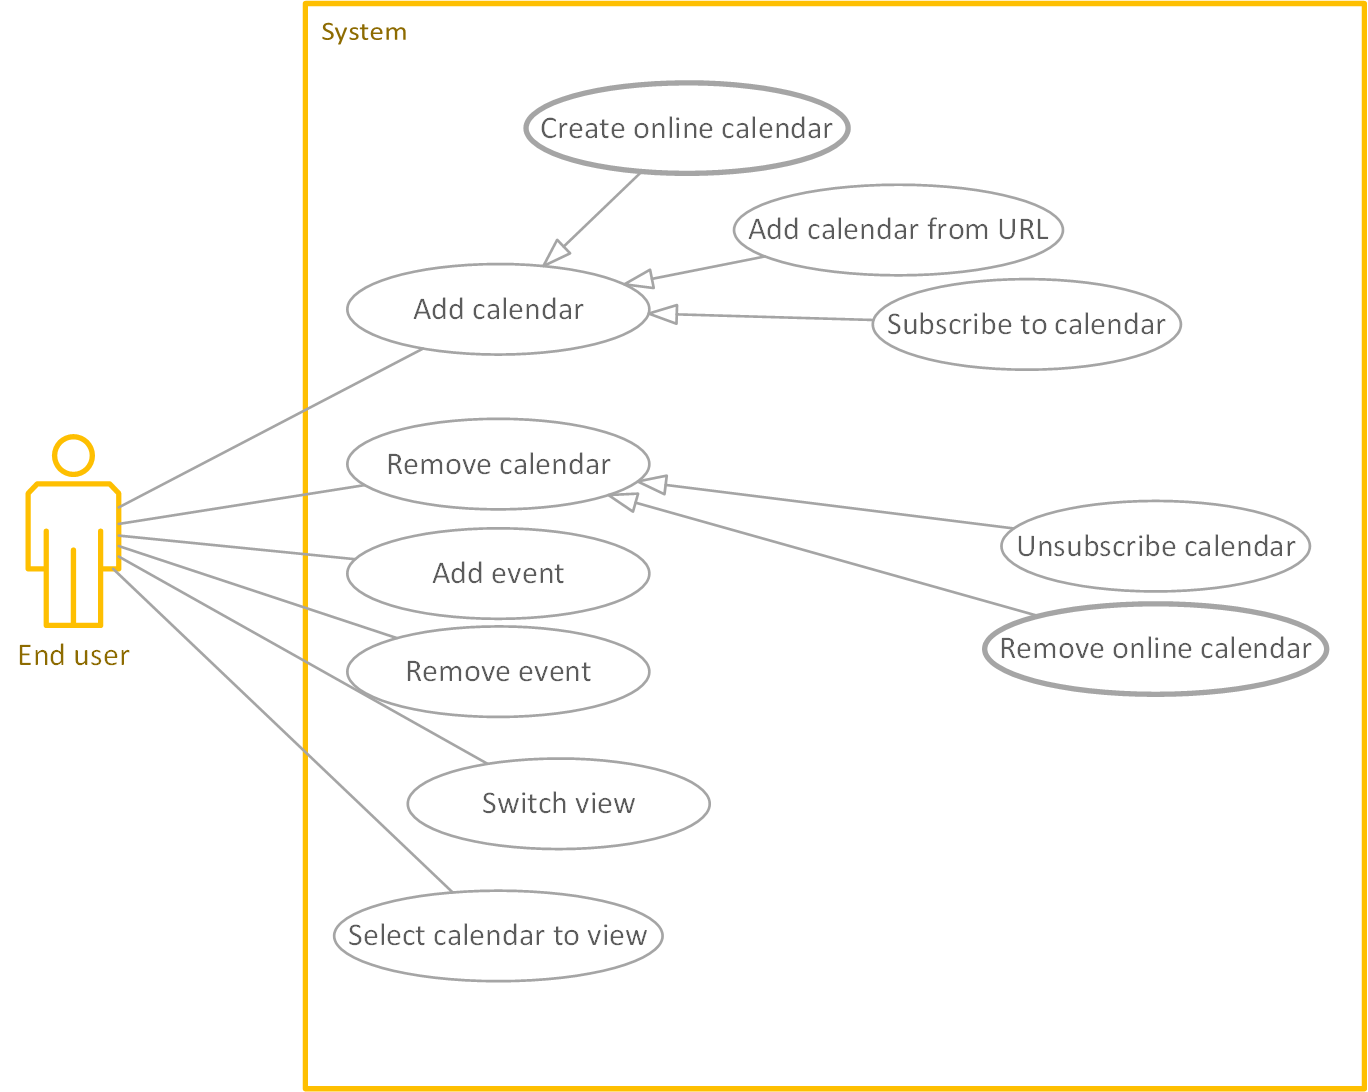
\includegraphics[scale=0.8]{figures/use_case_diagram.png}
\end{figure}

\subsubsection{Non-trivial use cases}
\begin{table}[H]
\noindent \textbf{Subscribe calendar}\\
\begin{tabularx}{\textwidth}{l X}
\midrule
\textit{Use case name} & SubscribeCalendar \\ \midrule
\textit{Participating actor} & Initiated by User \\ \midrule
\textit{Flow of events} & \tabitem User clicks the add calendar button\\
                                       & \tabitem User selects to add a
                                       subscription based calendar from the add
                                       calendar event\\
                                       & \tabitem User types calendar identifier \\
                                       & \tabitem User can now view added calendar events
                                       in client\\
                        \midrule
\textit{Entry condition} & User clicks add calendar.\\ \midrule
\textit{Exit condition} & \tabitem When user has successfully added a calendar. \\
						& \tabitem User cancels the operation.\\
                        \midrule
\end{tabularx}
\end{table}

\begin{table}[H]
\noindent \textbf{Add event}\\
\begin{tabularx}{\textwidth}{l X}
\midrule
\textit{Use case name} & AddEvent \\ \midrule
\textit{Participating actor} & Initiated by User \\ \midrule
\textit{Flow of events} & \tabitem User clicks the add event button\\
                                       & \tabitem User selects a calendar where
                                       the event will be added.\\
                                       & \tabitem User types details for event, such as
                                       name, place, note.\\
                                       & \tabitem User can now view event in selected calendar.\\
                        \midrule
\textit{Entry condition} & User clicks add event.\\ \midrule
\textit{Exit condition} & \tabitem When user has successfully added  an event. \\
						& \tabitem User cancels the operation.\\
                        \midrule
\end{tabularx}
\end{table}

\begin{table}[H]
\noindent \textbf{Remove event}\\
\begin{tabularx}{\textwidth}{l X}
\midrule
\textit{Use case name} & RemoveEvent \\ \midrule
\textit{Participating actor} & Initiated by User \\ \midrule
\textit{Flow of events} & \tabitem User clicks an event\\
                                       & \tabitem User selects remove/delete
                                       event from context menu.\\
                                       & \tabitem Users even has now been removed.\\
                        \midrule
\textit{Entry condition} & User clicks an event.\\ \midrule
\textit{Exit condition} & \tabitem When user has successfully removed an event. \\
						& \tabitem User cancels the operation.\\
                        \midrule
\end{tabularx}
\end{table}

%\subsubsection{Use case model}
\subsubsection{Object model}
\subsubsection{Initial Analysis Objects}
%%%%% Table 4-2 er på side 145 %%%%%
\begin{table}[H]
\begin{tabularx}{\textwidth}{l X}
\midrule
\textbf{User} & The user that interacts with the system. Main function is adding
  \texttt{Event}s and \texttt{Calendar}s. Removal is also included.\\ \midrule
\textbf{Calendar} & A \texttt{Calendar} holds the events for a given
  \texttt{User}. It can either be created by a \texttt{User} manually, or be
  provided via an URL for subscription from another \texttt{user}. \\ \midrule
\textbf{Event} & A \texttt{User} is able to add an event to his
  \texttt{Calendar}. An event can only be added to a user's own calendar. An event can also be removed, and again only by a user, who made calendar.\\ \midrule
\end{tabularx}
\end{table}

% Static model
% Static model

\subsubsection{Dynamic model}
% Dynamic model

%\subsubsection{User interface}

%\section{Glossary}

\end{document}
